\documentclass[xetex,mathserif,serif]{beamer}
\usepackage{polyglossia}
\setdefaultlanguage[babelshorthands=true]{russian}
\usepackage{minted}
\usepackage{tabu}

\useoutertheme{infolines}

\usepackage{fontspec}
\setmainfont{FreeSans}
\newfontfamily{\russianfonttt}{FreeSans}

\setbeamertemplate{blocks}[rounded][shadow=false]

\definecolor{links}{HTML}{2A1B81}
\hypersetup{colorlinks,linkcolor=,urlcolor=links}

\tabulinesep=0.7mm

\newcommand{\attribution}[1] {
    \vspace{-5mm}\begin{flushright}\begin{scriptsize}\textcolor{gray}{\textcopyright\, #1}\end{scriptsize}\end{flushright}
}

\title{Практика 4: моделирование структуры}
\author[Юрий Литвинов]{Юрий Литвинов \newline \textcolor{gray}{\small\texttt{yurii.litvinov@gmail.com}}}

\date{07.02.2022}

\begin{document}
    
    \frame{\titlepage}

    \section{Диаграммы классов}

    \begin{frame}
        \frametitle{Диаграммы классов}
        \begin{center}
            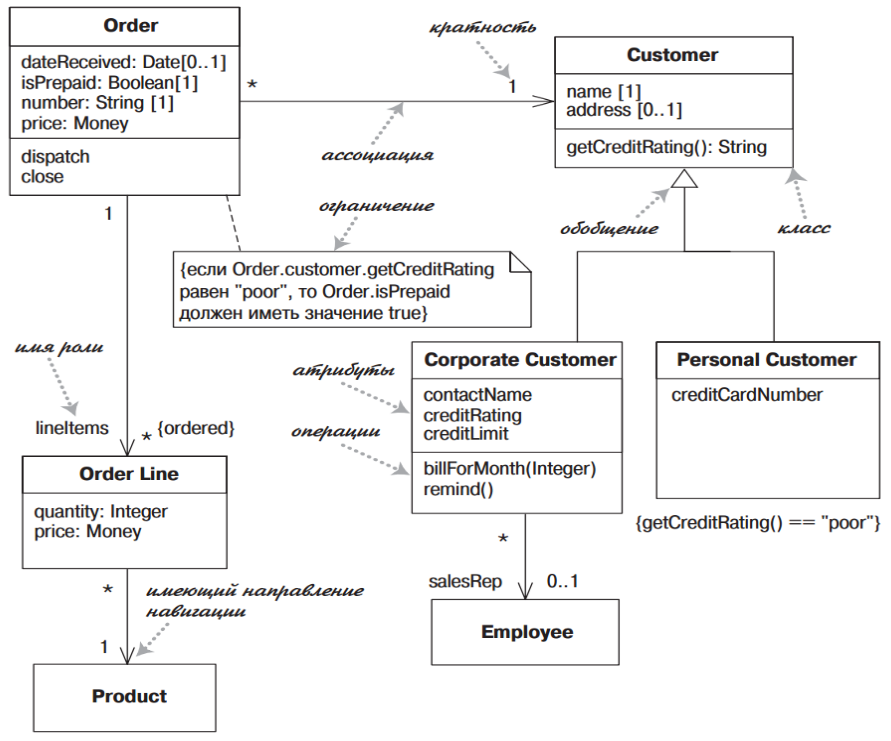
\includegraphics[width=0.7\textwidth]{umlClassDiagram.png}
        \end{center}
    \end{frame}

    \begin{frame}
        \frametitle{Свойства}
        \begin{columns}
            \begin{column}{0.3\textwidth}
                \begin{center}
                    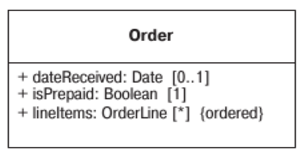
\includegraphics[width=0.8\textwidth]{attributes.png}

                    Атрибуты
                \end{center}
            \end{column}
            \begin{column}{0.7\textwidth}
                \begin{center}
                    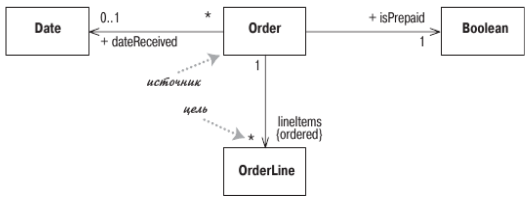
\includegraphics[width=0.7\textwidth]{associations.png}

                    Ассоциации
                \end{center}
            \end{column}
        \end{columns}
        \bigskip
        \begin{itemize}
            \item Не надо рисовать связи с enum-ами
            \item Если нарисовали связь, не пишите атрибут внутри класса
            \item Если поле два, рисуйте две ассоциации
            \item Не стесняйтесь именовать роли, указывать множественности и т.п
        \end{itemize}
    \end{frame}

    \begin{frame}
        \frametitle{Агрегация и композиция}
        Агрегация:
        \begin{center}
            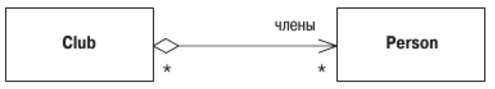
\includegraphics[width=0.5\textwidth]{aggregations.png}
        \end{center}
        Композиция:
        \begin{center}
            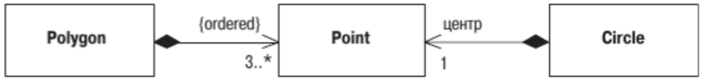
\includegraphics[width=0.7\textwidth]{compositions.png}
        \end{center}
        Уточнение обычной ассоциации, используется только если очень надо
    \end{frame}

    \begin{frame}
        \frametitle{Прочее}
        \begin{columns}
            \begin{column}{0.5\textwidth}
                \begin{center}
                    Интерфейсы

                    \bigskip
                    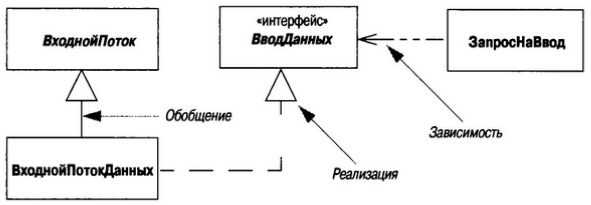
\includegraphics[width=0.9\textwidth]{interfaces1.png}

                    \bigskip
                    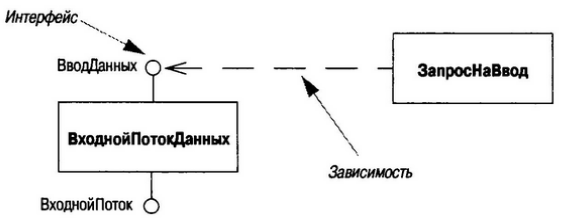
\includegraphics[width=0.9\textwidth]{interfaces2.png}
                \end{center}
            \end{column}
            \begin{column}{0.5\textwidth}
                \begin{center}
                    Зависимости

                    \bigskip
                    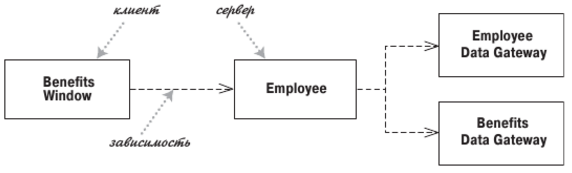
\includegraphics[width=0.9\textwidth]{dependencies.png}
                    \bigskip

                    Шаблоны

                    \bigskip
                    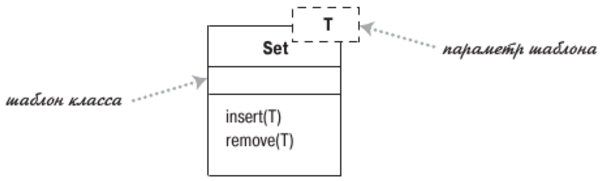
\includegraphics[width=0.9\textwidth]{templates.png}
                \end{center}
            \end{column}
        \end{columns}
    \end{frame}

    \section{Диаграммы компонентов}
    
    \begin{frame}
        \frametitle{Диаграммы компонентов}
        \begin{center}
            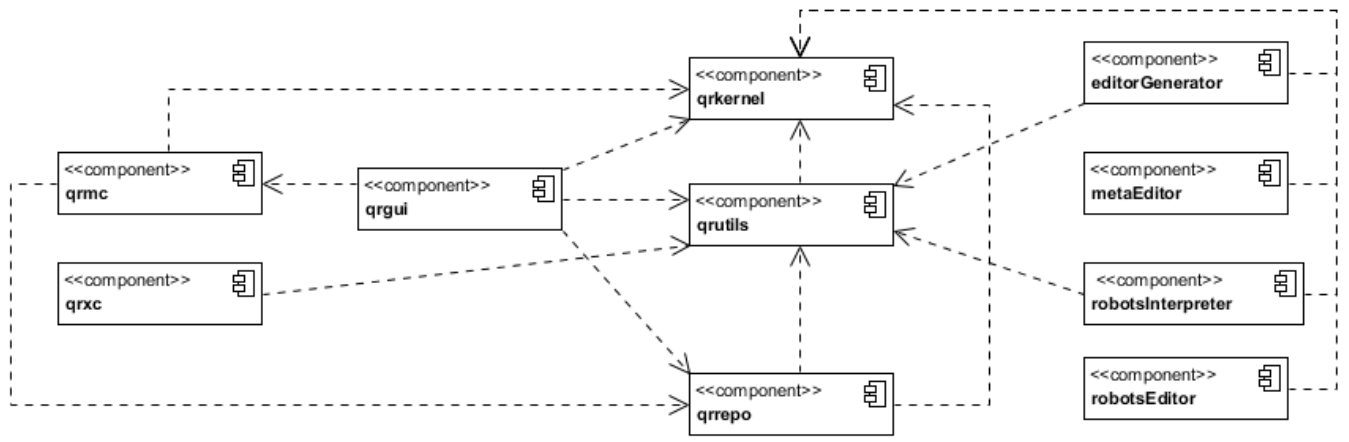
\includegraphics[width=0.95\textwidth]{componentDiagrams.png}
        \end{center}
    \end{frame}

    \begin{frame}
        \frametitle{Более подробно}
        \begin{center}
            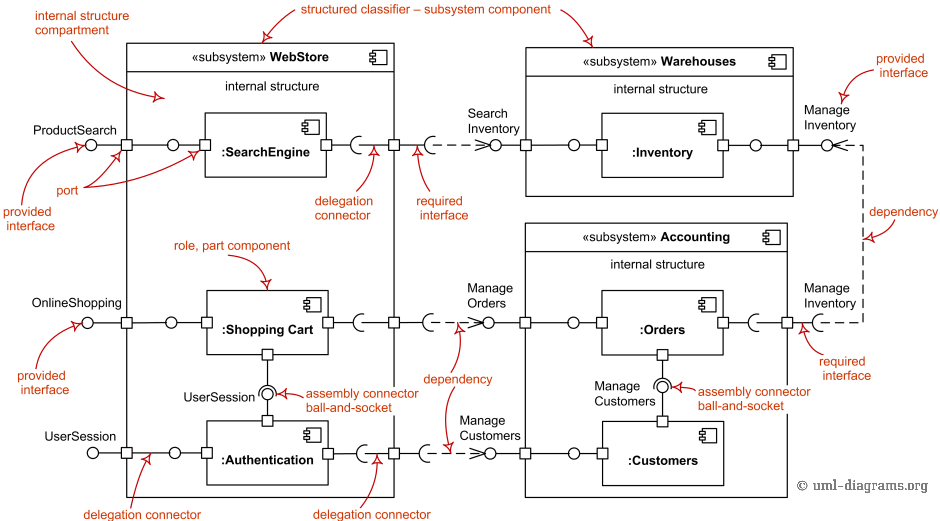
\includegraphics[width=0.95\textwidth]{componentDiagramsOverview.png}
            \attribution{\url{http://www.uml-diagrams.org}}
        \end{center}
    \end{frame}

    \section{Диаграммы развёртывания}
    
    \begin{frame}
        \frametitle{Диаграммы развёртывания}
        \framesubtitle{Диаграммы размещения}
        \begin{columns}
            \begin{column}{0.5\textwidth}
                \begin{itemize}
                    \item Показывает отображение компонентов и физических артефактов на реальные (или виртуальные) устройства
                    \item Бывает полезна на начальных этапах проектирования, даже до диаграмм компонентов
                \end{itemize}
            \end{column}
            \begin{column}{0.5\textwidth}
                \begin{center}
                    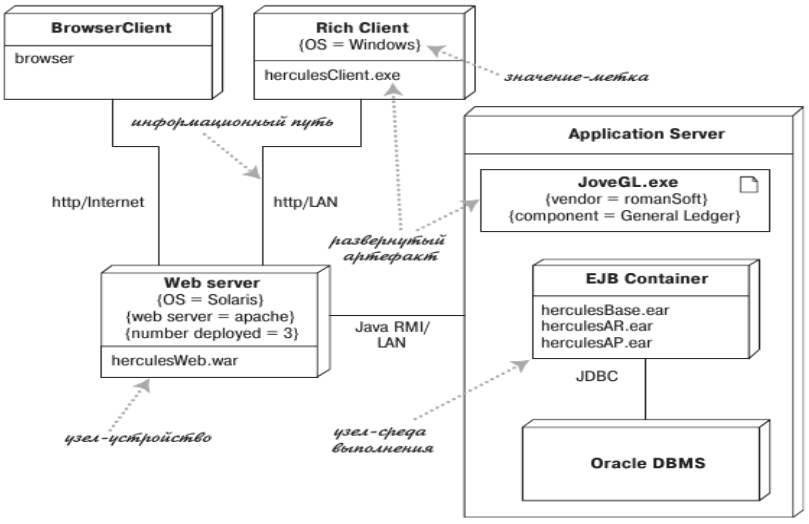
\includegraphics[width=\textwidth]{deploymentDiagram.png}
                    \attribution{М. Фаулер, UML. Основы}
                \end{center}
            \end{column}
        \end{columns}
    \end{frame}

    \section{Задания}

    \begin{frame}
        \frametitle{Задание на остаток пары}
        Вспомнить запрос \url{https://bit.ly/defects-rfp}, построить по нему:
        \begin{enumerate}
            \item диаграмму классов, моделирующую данные, хранимые системой
            \item диаграмму компонентов требуемой системы, как вы её видите
            \item диаграмму развёртывания, как вы её видите
            \begin{itemize}
                \item с указанием компонентов, разворачиваемых на узле
            \end{itemize}
        \end{enumerate}
    \end{frame}

\end{document}